% Created 2020-07-28 Tue 19:55
% Intended LaTeX compiler: pdflatex
\documentclass[letter]{article}
\usepackage[utf8]{inputenc}
\usepackage[T1]{fontenc}
\usepackage{graphicx}
\usepackage{grffile}
\usepackage{longtable}
\usepackage{wrapfig}
\usepackage{rotating}
\usepackage[normalem]{ulem}
\usepackage{amsmath}
\usepackage{textcomp}
\usepackage{amssymb}
\usepackage{capt-of}
\usepackage{hyperref}
\usepackage{multicol}
\usepackage[margin=1.3in]{geometry}
\setlength{\columnsep}{1cm}
\usepackage{palatino}
\fontfamily{ppl}\selectfont
\usepackage[spanish, es-noindentfirst]{babel}
\usepackage{setspace}
\setstretch{1.5}
\usepackage{fancyhdr}
\fancyhf{}
\pagestyle{fancy}
\lhead{\hleft}
\rhead{\hright}
\cfoot{\thepage}
\renewcommand{\headrulewidth}{1pt}
\renewcommand{\footrulewidth}{0pt}
\newcommand{\hleft}{Clasificación morfológica foliar}
\newcommand{\hright}{INF 324}
\author{Jesus Izurieta Veliz \quad Cristian Aquino Apaza}
\date{\today}
\title{Clasificación morfológica foliar mediante procesamiento de imágenes}
\hypersetup{
 pdfauthor={Jesus Izurieta Veliz \quad Cristian Aquino Apaza},
 pdftitle={Clasificación morfológica foliar mediante procesamiento de imágenes},
 pdfkeywords={},
 pdfsubject={},
 pdfcreator={Emacs 26.3 (Org mode 9.4)}, 
 pdflang={Spanish}}
\begin{document}

\maketitle
\begin{abstract}
El reconocimiento de objetos en imágenes y su clasificación es un problema
ampliamente estudiado en la actualidad, y cuando es necesario aplicarlo, en
general suele pensarse en una solución que implemente redes neuronales y una
gran cantidad de imágenes de prueba para entrenarlas, sin embargo, en algunos
casos específicos, este problema puede tener soluciones más sencillas y rápidas
de implementar. En este caso estudiamos el problema de la clasificación
morfológica de hojas de plantas, sin recurrir al uso de redes neuronales y con un
número reducido de imágenes de prueba.
\end{abstract}


\section{Introducción}
\label{sec:org910a519}
Las redes neuronales son en general una solución eficiente para el problema de
reconocimiento de objetos en imágenes, especialmente en casos en que el objeto
que se quiere obtener de una imagen puede encontrarse en muchas posiciones y
tener una gran cantidad de variaciones, para lo cual es necesaria una gran
cantidad de imágenes de prueba de modo que la red neuronal pueda entrenarse y
responder apropiadamente a una gran cantidad de situaciones. En este caso, el
problema que tratamos de resolver es de una complejidad menor y puede resolverse
por otros medios.

Para clasificar la hoja de una planta, necesitamos una forma de representar su
forma, en este punto nos será útil el método de momentos invariantes de Hu, que
genera valores que describen la forma de un objeto si tenemos su silueta. Los
momentos invariantes de Hu funcionan correctamente en objetos en dos dimensiones
y pueden darnos valores de una imagen que no varían ante transformaciones
simples como escalado o rotación, sin embargo, no nos serán útiles para
transformaciones en tres dimensiones, por lo tanto, su aplicación en este
problema lo convierte en una buena opción, ya que en general, para observar
correctamente la hoja de una planta, suele acomodársela de modo que su forma se
puede observar claramente.

Como un proceso previo a la clasificación de una hoja por la forma que tiene,
tendremos que encontrar la manera de obtener su silueta de la forma más limpia
posible, por lo que utilizamos también técnicas de preprocesado de imágenes como
binarización de imágenes Otsu, que nos permite separar objetos en una imagen
según la disposición del histograma de la imagen.

\subsection{Objetivos}
\label{sec:orgae5198c}
\subsubsection{Objetivo general}
\label{sec:org1fe9831}
\begin{itemize}
\item Desarrollo de una biblioteca para reconocer y clasificar hojas de plantas en
imágenes sin hacer uso de métodos avanzados de inteligencia artificial como
redes neuronales.
\end{itemize}

\subsubsection{Objetivos específicos}
\label{sec:org54f65e9}
\begin{itemize}
\item Desarrollo de una biblioteca que permita una cómoda manipulación de imágenes
para su procesamiento.
\item Expansión de la biblioteca de procesamiento de imágenes implementando
diferentes algoritmos de preprocesamiento de imágenes.
\item Desarrollo de un notebook destallando paso a paso el uso de la biblioteca para
este caso específico.
\end{itemize}

\section{Metodología}
\label{sec:org69e0479}
Este trabajo constituye un análisis descriptivo de la aplicación de diversos
métodos de procesamiento de imágenes, que son aplicados a este problema
específico para comprobar sus resultados. Se parte de la hipótesis inductiva de
que las técnicas usadas nos servirán para conseguir los objetivos de este
proyecto. Estas técnicas que fueron diseñadas para diferentes etapas del
procesamiento de imágenes, pueden aplicarse secuencialmente, ya que cada una
corresponde a una tarea específica que será complementada por las demás.

Seguimos entonces una secuencia de acciones con la finalidad de cumplir el
objetivo de clasificar una hoja en una imagen digital, siguiendo los pasos como
se muestra a continuación:

\begin{center}
\textbf{Binarización de la imagen} \(\rightarrow\) \textbf{Descripción morfológica} \(\rightarrow\)
 \textbf{Clasificación} \(\rightarrow\) \textbf{Comparación}
\end{center}

Cada uno de estos pasos implementa de forma independiente una técnica de
procesamiento de imágenes, por lo tanto, la imagen de prueba pasará de forma
secuencial por cada uno de estos procesos, siendo la salida de uno, la entrada
del siguiente.

El proceso de binarización de una imagen nos permite separar los objetos de
interés de una fotografía, para esto usamos la técnica de filtrado Otsu, que
analiza el histograma de la imagen encontrando un punto medio desde el cual
podremos separar grupos de objetos por colores. Para la descripción morfológica,
usamos momentos invariantes de Hu, una técnica que permite describir la forma de
una imagen mediante valores numéricos que no varían ante transformaciones
simples como escalado o rotación. Se analizan estadísticamente dos momentos de
Hu (\(\phi_1\) y \(\phi_2\)) para cada tipo de hoja de un conjunto de imágenes de
prueba, con la finalidad de poder determinar áreas en el plano \(\phi_1\), \(\phi_2\)
en que se encuentre cada tipo de hoja. Finalmente comparamos la posición en el
plano de los momentos obtenidos de una imagen para poder clasificarla en uno de
estos grupos con cierta probabilidad de pertenencia según su distancia al
centro de gravedad de cada conjunto.

\section{Morfología foliar}
\label{sec:org1ae6688}
La morfología foliar es una disciplina que clasifica las hojas de las plantas
por la forma que tienen, pueden clasificarse según diferentes atributos como la
forma del limbo, tipos de ápices foliares, tipos de bases, tipos de vernación y
nerviación y si son o no compuestas.

En la figura \ref{fig:org882cb80} se pueden apreciar las diferentes partes por las que las
hojas son clasificadas. En este trabajo, por simplicidad, tomamos en cuenta sólo
la clasificación por la forma del limbo en hojas simples, de modo que
distinguiremos las siguientes formas:

\begin{itemize}
\item lanceolada
\item flabelada
\item acumitada
\item orbicular
\item romboide
\item ovada
\item astada
\item palmeada
\item sagitada
\end{itemize}

\begin{figure}[htbp]
\centering
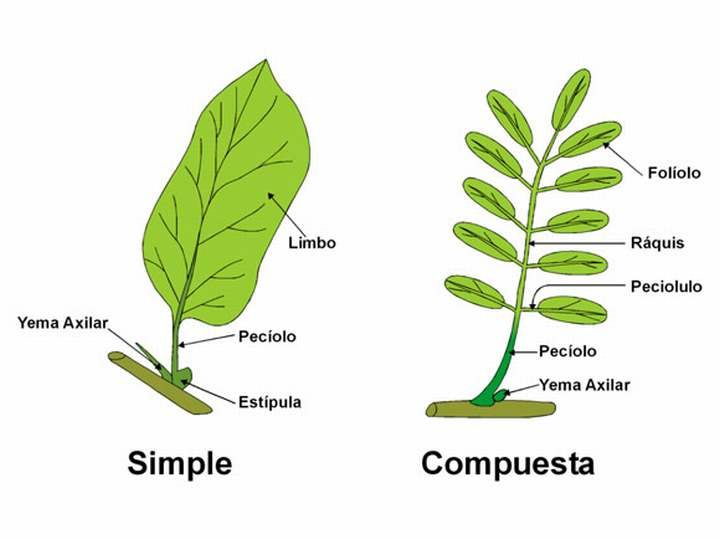
\includegraphics[width=.9\linewidth]{./images/leaf-parts.jpg}
\caption{\label{fig:org882cb80}Partes de una hoja.}
\end{figure}

\section{Desarrollo}
\label{sec:org407ec27}
Para este proyecto desarrollamos una librería que nos ayude a manipular una
imagen, proveyendo las funciones de convolución, modificación píxel a píxel,
histograma, cargado de imágenes y la capacidad de convertirlas en matrices y
viceversa, además de implementar los filtros necesarios para clasificar
imágenes.

El proyecto no contará con una interfaz gráfica, sino que constará de un
notebook interactivo de jupyter en el que se podrá apreciar tanto el código
fuente como los resultados de cada paso del proceso de manipulado de las
imágenes.

\subsection{Representación de imágenes}
\label{sec:org1679595}
Primeramente definiremos algunos conceptos que utilizaremos en el desarrollo del
proyecto. Para el tratamiento de una imagen digital, la representaremos como una
función de la posición de sus pixeles como sigue:

$$ I:\mathbb N^2 \rightarrow [0, 1] $$
$$ I(x, y) $$

Donde el rango representa el nivel de luminosidad para los pixeles en
coordenadas x e y en el caso de imágenes en escala de grises, para imágenes a
color, tendremos en su lugar una tupla de tres elementos, uno para cada uno de
los colores rojo, verde y azul. En el caso de una imagen digital, estos valores
varían en el rango \([0,255]\in \mathbb N\).

\subsection{Manipulación de imágenes}
\label{sec:org8fde29a}
La clase imagen es una abstracción básica que nos permitirá acceder y manipular
fácilmente una imagen que puede ser cargada desde un archivo, o puede ser creada
desde un array y posteriormente mostrada en un notebook de jupyter.

\begin{description}
\item[{Load file:}] (Parámetros: ruta) Carga en la instancia la imagen que se
encuentra en la ruta y la convierte en una matriz de tuplas de 3 componentes,
uno por cada color RGB, almacenándola en el atributo \texttt{array} de la clase
imagen, además define otros atributos como las dimensiones de la imagen.

\item[{Load array:}] (Parámetros: array) Almacena una matriz en el atributo \texttt{array}
de la imagen, la matriz debe ser contener tuplas de tres valores que se
encuentren entre 0 y 255.

\item[{Show:}] Retorna un objeto PIL.Image.Image que permite visualizar la imagen en
un notebook de jupyter o almacenarla como un archivo.

\item[{I:}] (Parámetros: x, y) Representa la función \(I(x, y)\) definida previamente,
retorna los píxeles en la posición x, y como una tupla de 3 valores.

\item[{I normal:}] (Parámetros: x, y) Igual que I() pero en lugar de retornar
valores en el rango [0, 255] normaliza los valores al rango [0, 1].

\item[{I m:}] (Parámetros: x, y, color) Igual que I(), pero retorna un único valor
definido por el parámetro \texttt{color}, 0 para rojo, 1 para verde y 2 para azul, el
valor por defecto es rojo si no se define el parámetro color.

\item[{I mnormal:}] (Parámetros: x, y, color) Igual que I\textsubscript{m}() pero con valores
normalizados en el rango \([0, 1]\).

\item[{Iterator:}] Retorna un iterador de tuplas x, y que facilita iteraciones
sobre cada píxel de la imagen.

\item[{Map over:}] (Parámetros: func) Permite sobreescribir píxeles mediante una
función que se envía como parámetro, la función recibirá una tupla de 3
valores y debe devolver una tupla de 3 valores. Esta función nos permitirá
recorrer la totalidad de la imagen aplicando en cada pixel la función \texttt{func},
por ejemplo el código \texttt{img.map\_over(lambda x, y, z: (x, x, x))} ejecutado
sobre una imagen img2, permitirá cambiar el valor de cada canal por su valor
rojo, lo que convertirá a la imagen a blanco y negro.
\end{description}

\subsection{Procesamiento}
\label{sec:org413809c}
El procesamiento de una imagen para su posterior clasificación, consiste en la
separación de la parte de interés de la imagen (en este caso la hoja), de modo
que pueda apreciarse su forma sin objetos de fondo, esto se realizará usando el
método de filtrado de Otsu, posteriormente se obtendrán los momentos invariantes
de Hu de la imagen, que describen la forma que tiene la hoja.

\subsubsection{Segmentación de umbral de Otsu}
\label{sec:orgd8d7442}
La segmentación de una imagen por el método de Otsu consiste en separar un
objeto en una imagen de otros objetos que no nos son de interés, para esto
trabajamos sobre el histograma de una imagen, que representa la frecuencia en
que aparecen los colores en una imagen, un ejemplo de histograma separado por
colores rojo, verde y azul se puede ver en la figura \ref{fig:orgac0601c}

\begin{figure}[htbp]
\centering
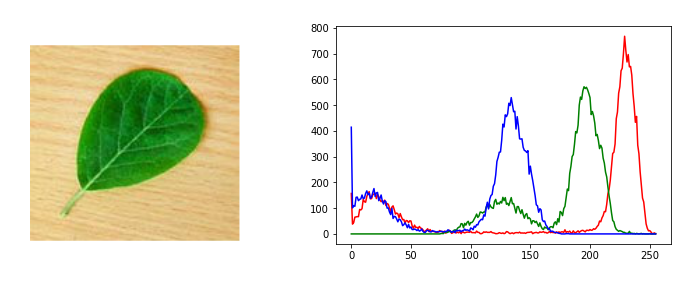
\includegraphics[width=.9\linewidth]{./images/histogram1.png}
\caption{\label{fig:orgac0601c}Histogramas por color en una imagen.}
\end{figure}

El problema de la segmentación de objetos en una imagen es un problema de
minimización, cuando encontramos una imagen en que el objeto de interés tiene un
color diferente al color de fondo, el histograma de la imagen toma una
disposición bimodal como se muestra en la figura \ref{fig:org58ed9c2}, trabajaremos con
imágenes convertidas a blanco y negro para tener un único histograma en el que
realizar la separación.

\begin{figure}[htbp]
\centering
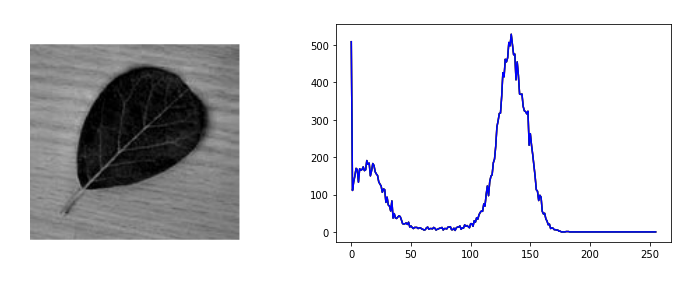
\includegraphics[width=.9\linewidth]{./images/histogram2.png}
\caption{\label{fig:org58ed9c2}Histograma de la imagen en blanco y negro, se puede apreciar un valle entre los valores 50 a 100 que separa dos grupos de colores.}
\end{figure}

Como se ve en la imagen \ref{fig:org58ed9c2}, el histograma bimodal tiene una clara
reparación en la que podemos separar dos grupos de colores, el punto de
separación se encontrará en el punto mínimo de ese valle, una vez encontrado
este punto, podemos binarizar la imagen separándola por umbrales, de modo que el
resultado es algo similar a la figura \ref{fig:org294a3e9}.

\begin{figure}[htbp]
\centering
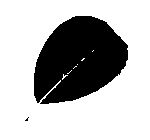
\includegraphics[width=5cm]{./images/binaryleaf.png}
\caption{\label{fig:org294a3e9}Imagen binarizada tomando el valor 75 para separar los umbrales de color.}
\end{figure}

La finalidad del método de Otsu es encontrar este punto mínimo en que la
separación de umbrales de color es óptima, esto se consigue encontrando el valor
\(t\) que minimiza la función:

\begin{equation}
\label{eq:org665e002}
\sigma_w^2(t) =  q_1(t)\sigma_1^2(t) + q_2(t)\sigma_2^2(t)
\end{equation}

En esta función \(t\) es la variable que debe ser minimizada y representa el punto
medio que dividirá los dos umbrales. Las funciones \(q_1(t)\) y \(q_2(t)\)
representan la probabilidad de cada grupo se definen como sigue:

$$ q_1(t) = \sum_{i=1}^t P(i), \quad q_2(t) = \sum_{i=t+1}^I P(i) $$

Para obtener estos valores, necesitamos normalizar nuesto histograma de modo que
su área sea igual a 1 y de este modo se convierta en una función de probabilidad
para cada valor de píxel, esta función normalizada es \(P(i)\), lo que hacen las
funciones \(q_1(t)\) y \(q_2(t)\) es separar esta función en dos partes, una de 0 a
t y otra de t+1 hasta I que es en este caso es 255. Seguidamente obtenemos la
media de ambas clases:

$$ \mu_1(t) = \sum_{i=1}^t \frac{i P(i)}{q_1(t)} , \quad \mu_2(t) = \sum_{i=t+1}^I \frac{i P(i)}{q_2(t)} $$

Y después de obtener la media de ambas clases, calculamos su varianza.

$$ \sigma_1^2(t) = \sum_{i=1}^t [i-\mu_1(t)]^2 \frac{P(i)}{q_1(t)} , \quad \sigma_2^2(t) = \sum_{i=t+1}^I [i-\mu_2(t)]^2 \frac{P(i)}{q_2(t)} $$

Con las funciones de probabilidad \(q_1(t)\) y \(q_2(t)\) y con la varianza de
estas, podemos obtener la ecuación \ref{eq:org665e002}, que representa la varianza de
pesos por clase\footnote{Traducido de \emph{weighted within-class variance}.}. Tendremos ahora que minimizar esta función,
para esto, la solución más sencilla consiste en evaluar esta función para cada
valor de 0 a 255 y seleccionar el valor mínimo para t, ya que
computacionalmente, el cálculo de \(\sigma_w^2(t)\) para cada t no tiene mucha
complejidad.

Los métodos \texttt{minimum\_otsu} y \texttt{binarize} implementan esta técnica, \texttt{minimum\_otsu}
se ocupa de calcular el valor t que minimiza la varianza, y \texttt{binarize} cambia
los valores de los pixeles de la imagen, dependiendo si se encuentran a la
derecha o izquierda del valor t, dando como resultado, una imagen como la figura
\ref{fig:org294a3e9}. El código puede encontrarse en la sección \hyperref[sec:orgdf60c56]{Anexos}.

\subsubsection{Momentos invariantes de Hu}
\label{sec:org44b811c}
Para obtener un valor propio de la forma geométrica de un objeto en una imagen,
usaremos momentos invariantes de Hu, un conjunto de valores calculados en base a
la imagen, que nos permiten describir su forma y que permanecen constantes aún
cuando se aplican sobre la imagen transformaciones como rotada o escalado.

Los momentos de orden \((p+q)\) en dos dimensiones sobre una función de
distribución \(p(x, y)\) continua, son calculados mediante integrales de Riemman
como sigue:

$$ m_{pq} =  \int_{-\infty}^{\infty} \int_{-\infty}^{\infty} x^p y^q p(x, y)\,dx\,dy \quad p, q = 0, 1, 2, ... $$

En este caso, usaremos momentos centrales que se definen como sigue para una
función \(p(x, y)\) continua:

$$ \mu_{pq} = \int_{-\infty}^{\infty} \int_{-\infty}^{\infty} (x-\bar x)^p (y-\bar y)^q p(x, y)\, d(x-\bar x)\,d(y-\bar y) $$

donde:

$$ \bar x = \frac{m_{10}}{m_{00}}, \quad \bar y = \frac{m_{01}}{m_{00}} $$

son las coordenadas del centroide\footnote{Centro de gravedad.} del objeto en la imagen.

Sin embargo, ya que se trata de una imagen digital en que usamos valores
discretos, calcularemos los momentos centrales con las ecuaciones:

$$
\mu_{pq} = \sum_x \sum_y x^p y^q I(x, y)
$$

$$ n_{pq} = \frac{\mu_{pq}}{\mu_{00}^r}, \quad r=\frac{p+q}{2}+1 $$

Con estas ecuaciones podremos calcular los momentos invariantes que usaremos en
este proyecto. Nos limitamos a usar los primeros dos momentos invariantes de Hu,
ya que nos son suficientes en este caso.

$$ \phi_1 = n_{20} + n_{02}, \quad \phi_2 = (n_{20} + n_{02})^2 + 4n_{11}^2 $$

Estos dos valores representan la extensión y la estrechez del objeto
respectivamente\footnote{Traducido de \emph{spread} y \emph{slenderness} en el artículo original.}.
Este proceso es implementado en el método \texttt{hu\_moments} de la clase image,
retornando los dos primeros momentos.

\begin{figure}[htbp]
\centering

\includegraphics[width=.9\linewidth]{./images/stars.png}
\caption{\label{fig:org1b3252e}Imagen de una estrella con transformaciones, primero la imagen original, luego escalada, luego rotada y finalmente escalada y deformada.}
\end{figure}

Probando el algoritmo con las tres imágenes de ejemplo de la figura \ref{fig:org1b3252e} obtenemos
los valores:

\begin{center}
\begin{tabular}{lrr}
 & \(\phi_1\) & \(\phi_2\)\\
\hline
Imagen 1 & 0.2162437035817964 & 7.15421105863606e-10\\
Imagen 2 & 0.21685851808651274 & 4.778874641818779e-09\\
Imagen 3 & 0.2162170223369867 & 6.370439738565976e-09\\
Imagen 4 & 0.23248362379752913 & 0.007129570200901847\\
\end{tabular}
\end{center}

Los valores de \(\phi_1\) y \(\phi_2\) para las primeras tres transformaciones son
muy similares debido a que se trata de la misma forma en diferentes tamaños y
posiciones, mientras que los momentos de la imagen 4 varían notablemente por
estar deformada.

\subsection{Datos de comparación}
\label{sec:org33022ec}
Para obtener datos de comparación, recolectamos algunas imágenes de ejemplo que
nos servirán para tener valores iniciales de momentos invariantes para
diferentes tipos de hojas (Figura \ref{fig:org02b0811}).

\begin{figure}[htbp]
\centering
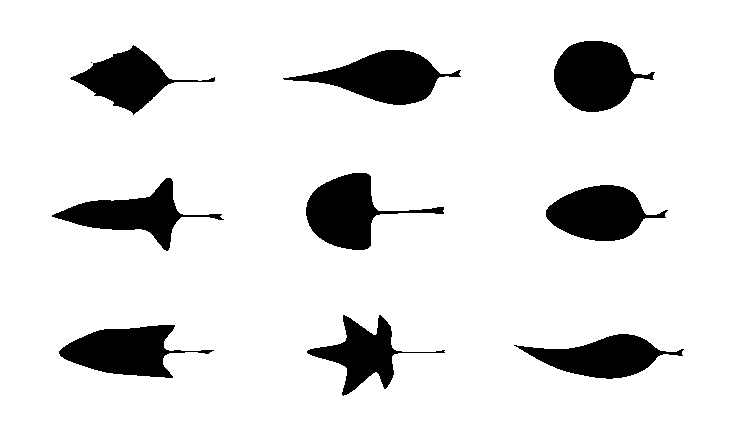
\includegraphics[width=.9\linewidth]{./images/leaves.png}
\caption{\label{fig:org02b0811}Imágenes de prueba de los tipos de hojas que clasificamos.}
\end{figure}

Aplicando las técnicas de filtrado de Otsu y momentso invariantes de Hu, obtenemos los valores de \(\phi_1\) y \(\phi_2\) para las imágenes de prueba.

\begin{table}[htbp]
\caption{Momentos invariantes obtenidos de las imágenes de ejemplo.}
\centering
\begin{tabular}{lrr}
\hline
Tipo de hoja & \(\phi_1\) & \(\phi_2\)\\
\hline
Lanceolada & 0.08241080043135868 & 0.3999693426853134\\
Flabelada & 0.02452288351987129 & 0.3207811493752293\\
Acumitada & 0.05055337469475332 & 0.3610066090495226\\
Orbicular & 0.020097387958003515 & 0.31300964425473893\\
Romboide & 0.04190473916737033 & 0.34816780188557916\\
Ovada & 0.023285971562215516 & 0.35150337160513034\\
Astada & 0.033590539033761975 & 0.3190729877395031\\
Palmeada & 0.012872876070329099 & 0.2860389435844065\\
Sagitada & 0.06468482190387434 & 0.4117437381830096\\
\hline
\end{tabular}
\end{table}

En la figura \ref{fig:org15ec368} podemos ver cómo se distribuyen los momentos de las imágenes en el plano.

\begin{figure}[htbp]
\centering
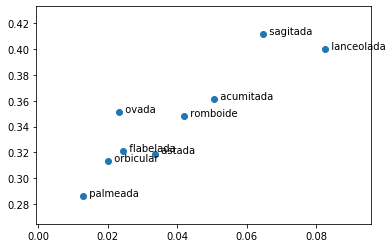
\includegraphics[width=10cm]{./images/moments.jpg}
\caption{\label{fig:org15ec368}Distribución de momentos invariantes por tipo de hoja en el plano \(\phi_1, \phi_2\).}
\end{figure}

\subsection{Comparación y clasificación}
\label{sec:org09dd806}
Para comparar los resultados de momentos de una imagen con valores obtenidos
previamente, el algoritmo ideal a ser utilizado es K-nearest neighbors.

\subsubsection{Algoritmo K-Nearest Neighbors}
\label{sec:org2a94bf7}
K-Nearest Neighbors, o KNN para abreviar, es uno de los algoritmos de
aprendizaje automático más simples y se utiliza en una amplia gama de
instituciones. KNN es un algoritmo de aprendizaje lento no paramétrico. Cuando
decimos que una técnica no es paramétrica, significa que no hace suposiciones
sobre los datos subyacentes. En otras palabras, realiza su selección en función
de la proximidad a otros puntos de datos, independientemente de la
característica que representen los valores numéricos.Ser un vago algoritmo de
aprendizaje implica que hay poca o ninguna fase de entrenamiento. Por lo tanto,
podemos clasificar inmediatamente los nuevos puntos de datos a medida que se
presentan.

Algunos pros y contras de KNN

\begin{enumerate}
\item Pros :
\label{sec:orgf432d73}
\begin{itemize}
\item No hay suposiciones sobre los datos.
\item Algoritmo simple - fácil de entender
\item Se puede usar para clasificación y regresión
\end{itemize}

\item Contras :
\label{sec:orgbc7ad4f}
\begin{itemize}
\item Requisito de memoria alta: todos los datos de entrenamiento deben estar
presentes en la memoria para calcular los K vecinos más cercanos
\item Sensible a características irrelevantes
\item Sensible a la escala de los datos ya que estamos calculando la distancia a los
puntos K más cercanos.
\end{itemize}
\end{enumerate}

\subsection{Ejecución y resultados}
\label{sec:org5a835cb}
Ahora procedemos a utilizar la biblioteca desarrollada con una imagen de ejemplo
que podremos clasificar. Primeramente importamos las bibliotecas que usaremos.

\begin{verbatim}
from image import Image
import matplotlib.pyplot as plt
\end{verbatim}

Cargaremos las imágenes de prueba que mostramos previamente en la figura
\ref{fig:org02b0811}.

\begin{verbatim}
lanceolada = "./testimages/leafs/lanceolada.jpg"
flabelada = "./testimages/leafs/flabelada.jpg"
acumitada = "./testimages/leafs/acumitada.jpg"
orbicular = "./testimages/leafs/orbicular.jpg"
romboide = "./testimages/leafs/romboide.jpg"
ovada = "./testimages/leafs/ovada.jpg"
astada = "./testimages/leafs/astada.jpg"
palmeada = "./testimages/leafs/palmeada.jpg"
sagitada = "./testimages/leafs/sagitada.jpg"

leafs =[lanceolada, flabelada, acumitada, orbicular, romboide, ovada, astada, palmeada, sagitada]
\end{verbatim}

Podemos abrir una de estas imágenes para comprobar que se hayan cargado correctamente:

\begin{verbatim}
ll = Image()
ll.load_file(flabelada)
ll.show()
\end{verbatim}

Nos mostrará la imagen:

\begin{center}
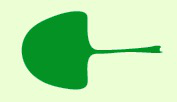
\includegraphics[width=.9\linewidth]{./images/show.png}
\end{center}

A continuación hacemos una copia de la imagen y calculamos sus momentos invariantes

\begin{verbatim}
lle = ll
bound = lambda x: 255 if x > 200 else 1
lle.map_over(lambda r, g, b: (bound(g), bound(g), bound(g)))
lle.show()
print(ll.hu_moments())
\end{verbatim}

\begin{center}
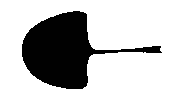
\includegraphics[width=.9\linewidth]{./images/showbn.png}
\end{center}

Como resultado obtenemos: \texttt{(0.29768184782794443, 0.021067187247205375)}.
Realizaremos este proceso de forma iterativa para cada una de las imágenes de
prueba, para esto desarrollamos las funciones  binarize y get\textsubscript{moments}.

\begin{verbatim}
def binarize_(url):
    ll = Image()
    ll.load_file(url)
    ll.map_over(lambda r, g, b: (bound(b), bound(b), bound(b)))
    return ll

binary_leafs = map(binarize_, leafs)
hu_moments = list(map(lambda x: x.hu_moments(), binary_leafs))

def get_moments(url):
    im = Image()
    im.load_file(url)
    return ("  "+url.split("/")[3].split(".")[0], im.hu_moments())

get_position = lambda x: x[1]
\end{verbatim}

De este modo podremos visualizar la distribución de los momentos invariantes de
las imágenes en el plano.

\begin{verbatim}
hu_name_moments = list(map(get_moments, leafs))
plt.scatter(*zip(*hu_moments))
for label, moments in hu_name_moments:
    plt.annotate(label, moments)
url, moments = get_moments(leafs[1])
plt.show()
\end{verbatim}

\begin{center}
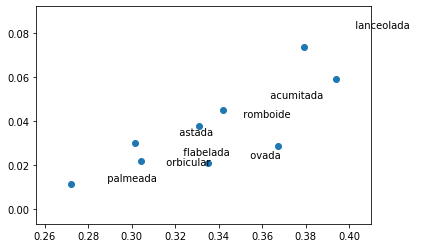
\includegraphics[width=.9\linewidth]{./images/plano.png}
\end{center}

Ahora cargamos la imagen de prueba que usaremos

\begin{verbatim}
test = "./testimages/leafs/test3.jpg"
testimage = Image()
testimage.load_file(test)
testimage.show()
\end{verbatim}

\begin{center}
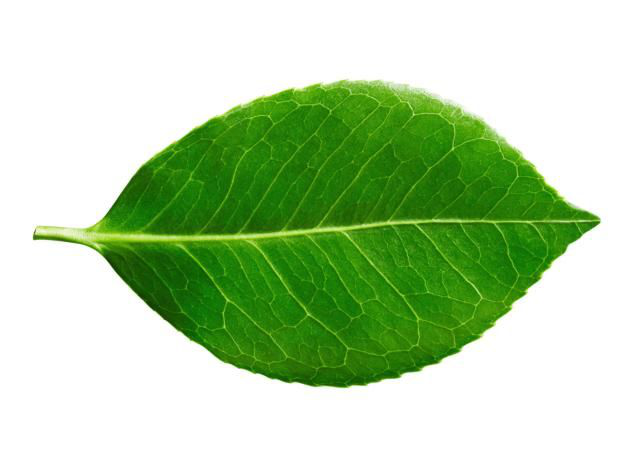
\includegraphics[width=.9\linewidth]{./images/test.png}
\end{center}

Convertimos la imagen a blanco y negro

\begin{verbatim}
testimage.black_white().show()

\end{verbatim}

\begin{center}
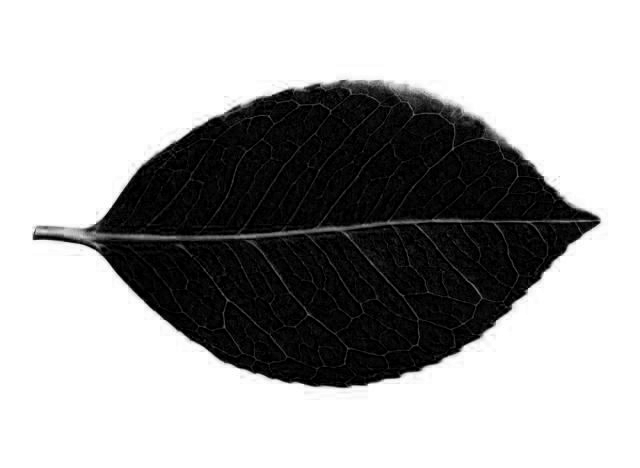
\includegraphics[width=.9\linewidth]{./images/testbn.png}
\end{center}

Y obtenemos su histograma

\begin{verbatim}
hist_normal = testimage.histogram()
plt.plot(hist_normal, 'g')
plt.show()
\end{verbatim}

\begin{center}
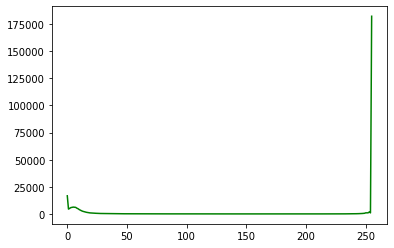
\includegraphics[width=.9\linewidth]{./images/hist.png}
\end{center}

Calculamos el valor t que minimiza la varianza

\begin{verbatim}
t = testimage.minimum_otsu()
print(t)

134
\end{verbatim}

Y lo usamos para binarizar la imagen

\begin{verbatim}
image = testimage.copy()
image.binarize(t).show()
\end{verbatim}

\begin{center}
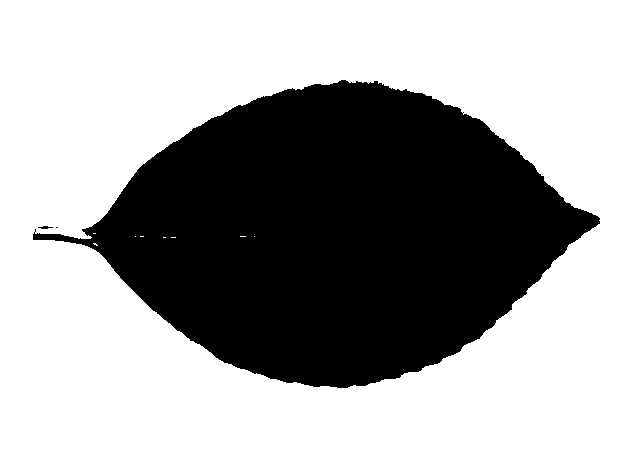
\includegraphics[width=.9\linewidth]{./images/testbin.png}
\end{center}

Calculamos los momentos de Hu de la imagen

\begin{verbatim}
hm = image.hu_moments()
print(hm)
\end{verbatim}

Y obtenemos \texttt{(0.3601956207386796, 0.010512156197008187)}.

Finalmente agregamos la imagen a la gráfica para comprobar sus cercanía con
otros valores.

\begin{verbatim}
hu_moments = list(map(get_position, hu_name_moments))
tm = ("imagen de prueba", hm)

plt.scatter(*zip(*hu_moments))
for label, moments in hu_name_moments:
    plt.annotate(label, moments)
plt.scatter(*hm)
plt.annotate(*tm)
url, moments = get_moments(leafs[1])
plt.show()
\end{verbatim}

\begin{center}
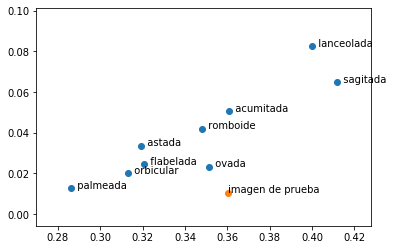
\includegraphics[width=.9\linewidth]{./images/result.png}
\end{center}

Finalmente comprobamos que a simple vista, la imagen se encuentra cerca de la
forma ovada, que es la forma correcta, sin embargo se encuentra algo alejada del
resultado, con más imágenes de prueba y un mejor preprocesamiento de la imagen
se podrían obtener mejores resultados.

\section{Referencias}
\label{sec:org5ca9fb5}

\section{Anexos}
\label{sec:orgdf60c56}
\subsection{Código fuente}
\label{sec:org4dbb867}
\begin{verbatim}
#!/usr/bin/env python3
import matplotlib.image as plt_img
import numpy as np
from PIL import Image as pil_image
from functools import reduce
from math import sqrt
from copy import deepcopy


class Image:

    def __init__(self):
        self.route = "."
        self.image = None
        self.array = None
        self.height, self.width, self.dat = (0,0,0)

    def load_file(self, route):
        self.route = route
        self.image = plt_img.imread(route)
        self.array = self.image.tolist()
        self.height, self.width, self.dat = self.image.shape

    def load_array(self, array):
        self.array = array
        self.height = len(array)
        self.width = len(array[0])

    def I(self, x, y):
        """ Devuelve rgb en x, y """
        return tuple(self.array[x][y])

    def I_m(self, x, y, color=0):
        """ Devuelve un color de x, y """
        triple = self.array[x][y]
        return triple[color]

    def I_normal(self, x, y):
        """ Devuelve rgb en [0, 1] """
        (i, j, k) = self.I(x, y)
        return (i/255, j/255, k/255)

    def I_mnormal(self, x, y, color=0):
        """ Devuelve color en [0, 1] """
        i = self.I_m(x, y, color)
        return i/255

    def show(self, route=None):
        if route:
            self.route = route
        image_arr = np.asarray(self.array, dtype="uint8")
        img_file = pil_image.fromarray(image_arr, 'RGB')
        return img_file

    def iterator(self):
        for i in range(self.height):
            for j in range(self.width):
                yield (i,j)

    def map_over(self, func):
        """ Ejecución de func sobre cada pixel """
        for x, y in self.iterator():
            self.array[x][y] = func(*self.I(x, y))

    def copy(self):
        return deepcopy(self)

    def crop(self, x1, y1, x2, y2):
        cropped_array = []
        for i in range(y1, y2):
            arr = []
            for j in range(x1, x2):
                arr.append(self.I(i, j))
            cropped_array.append(arr)
        cropped_image = Image()
        cropped_image.load_array(cropped_array)
        return cropped_image

    def black_white(self):
        self.map_over(lambda r, g, b: (min(r, g, b), min(r, g, b), min(r, g, b)))
        return self

    def hu_moments(self):
        """ Primeros dos momentos de Hu """
        def moment_pq(p, q):
            """ Momentos geométricos """
            sum = 0
            for x, y in self.iterator():
                sum += x**p * y**q * self.I_mnormal(x, y)
            return sum

        m00 = moment_pq(0, 0)
        m01 = moment_pq(0, 1)
        m11 = moment_pq(1, 1)
        m10 = moment_pq(1, 0)
        m20 = moment_pq(2, 0)
        m02 = moment_pq(0, 2)

        def central_moment_20(a, b, c):
            """ Momentos centrales """
            return (a-(b**2/c))/(c**2)

        n20 = central_moment_20(m20, m10, m00)
        n02 = central_moment_20(m02, m01, m00)
        n11 = central_moment_20(m11, sqrt(m10*m01), m00)

        self.X = n20+n02
        self.Y = (n20-n02)**2+4*(n11**2)

        return (self.X, self.Y)

    def color_histogram(self):
        histr = [0 for _ in range(256)]
        histg = [0 for _ in range(256)]
        histb = [0 for _ in range(256)]
        for x, y in self.iterator():
            r = self.I_m(x, y, 0)
            g = self.I_m(x, y, 1)
            b = self.I_m(x, y, 2)
            histr[r] += 1
            histg[g] += 1
            histb[b] += 1
        return (histr, histg, histb)

    def otsu(self):
        pass

    def histogram(self):
        # hist = [(x, 0) for x in range(255)]
        hist = [0 for _ in range(256)]
        for x, y in self.iterator():
            p = self.I_m(x, y)
            hist[p] += 1
        return hist

    def minimum_otsu(self):
        hist = self.histogram()
        hist_sum = sum(hist)
        P = list(map(lambda x: x/hist_sum, hist))
        # función de probabilidad
        q1 = lambda t: sum(P[0:t])
        q2 = lambda t: sum(P[t+1:256])
        # media
        u1 = lambda t: sum([(i * P[i]) / q1(t) for i in range(0, t)])
        u2 = lambda t: sum([(i * P[i]) / q2(t) for i in range(t+1, 256)])
        # varianza
        v1 = lambda t: sum([(i - u1(t))**2 * (P[i] / q1(t)) for i in range(0, t)])
        v2 = lambda t: sum([(i - u2(t))**2 * (P[i] / q2(t)) for i in range(t+1, 256)])
        # weighted variance
        vw = lambda t: q1(t) * v1(t) + q2(t) * v2(t)
        minor = 100000
        ret = 0
        for t in range(256):
            try:
                vwt = vw(t)
                if vwt < minor:
                    minor = vwt
                    ret = t
            except:
                pass
        return ret

    def binarize(self, center):
        bound = lambda x: 255 if x > center else 0
        self.map_over(lambda r, g, b: (bound(b), bound(b), bound(b)))
        return self
\end{verbatim}
\end{document}
